\graphicspath{{Fusion/}}
%\citet{akbari2012} discussed Langmuir turbulence using low-level radar data using a single high-speed EMCCD camera.
%\citet{dahlgren2013} gave relative estimates of flaming auroral behavior with an EMCCD camera and PFISR-based starting assumptions.
Fast EMCCD camera observations with ISR routinely show thin, highly dynamic aurora with temporal signatures characteristic of DAW aurora.
Shear plasma flows such as occur during reconnection launch Alfvén waves of wavenumber short enough to be seen in $\sim$ 10 degree field of view (FOV) cameras focused on a region about magnetic zenith.
During active solar times, substorms occur frequently enough that multiple Alfvénic aurora may be observed in a single night.
The following subsections describe the instruments and methods used to distinguish inverted-V aurora from the Alfvénic aurora associated with NEIALs.

\FloatBarrier
\subsection{Poker Flat ISR (PFISR)}\label{sec:fuspfisr}
PFISR produces several low-level data products including the complex analog-to-digital converter voltage samples.
At the time, access to the large files containing low-level PFISR data is by request, with radar data accumulating at $\sim \unit[1.5]{MB/s}$ during a typical experiment.
% data: Apr 14 2013  (468530486 + 224263860 + 224263860 + 187839490) bytes / 729 seconds = 1.516 MByte/sec
Madrigal PFISR high-level data products have integration times $\sim \unit[2]{min}$ versus \unit[10..100]{ms} cadence of the low-level PFISR data.
Long integration time is necessary for plasma parameter estimation since incoherent returns from the ionospheric volume target provide return signals far too weak to characterize from a single pulse.
An autocorrelation function (ACF) is built up from the incoherent electron and ion scatterers over tens of seconds.
Taking the Fourier transform of the ACF the power spectral density (PSD) is obtained, with a notional PSD from a quiet ionosphere shown in Figure~\ref{fig:isrmorph}(a).
An ACF fitting algorithm provides estimates of electron number density, electron and ion temperature and ion velocity.

These plasma parameter estimates break down when turbulent plasma leads to a breakdown in the parameter fitter, which expects PSDs having morphology similar to Figure~\ref{fig:isrmorph}(a).
Strong Langmuir turbulence \citep{akbari2012} leads to ISR spectrum like that depicted in Figure~\ref{fig:isrmorph}(b).
\begin{figure}\centering
    \includegraphics[width=0.8\columnwidth,trim=80 260 100 280,clip]{gfx/isr_thermal}

    \includegraphics[width=0.8\columnwidth,trim=80 260 100 270,clip]{gfx/isr_slt}

    \includegraphics[width=0.8\columnwidth,trim=80 260 100 270,clip]{gfx/isr_streamupflow}
    \caption{(a) Notional PFISR spectrum for quiet ionospheric conditions. 
    	(b) Notional PFISR spectrum under strong Langmuir turbulence. 
    	(c) Notional PFISR spectrum with streaming upflowing plasma.}
    \label{fig:isrmorph}
\end{figure}
Streaming upflows lead to ISR spectrum similar to the depiction in Figure~\ref{fig:isrmorph}(c).
The ISR fitter algorithm used in plasma parameter estimation assumes a single-Maxwellian distribution, which breaks down under turbulent conditions, leading to non-physical plasma parameter estimates.
Alfvénic aurora associated with this Langmuir turbulence leaves fingerprints in the auroral morphology HiST was designed to observe.

The PFISR complex vector $\mathbf{I}+j\mathbf{Q}$ sampled time series is obtained with revisit time as fast as \unit[75]{ms} \citep{akbari2012} for five-beam pattern experiments and may be pushed at least to \unit[19]{ms} \citep{michell2009} for single-beam position experiments.
For future measurements, new ISR plasma line receiver techniques \citep{vierinen2016} reduce plasma line sampling cadence to about \unit[200]{ms}.
Table~\ref{tab:cadence} summarizes the time sampling capability of PFISR.
\begin{table}\centering
    \caption{Instrument sample rates vs. resolution used in experiments.}\label{tab:cadence}
    \begin{tabular}{llll}
        \toprule
        Instrument Measurement Mode & Resolution & Cadence [ms] & Date\\
        \midrule
        PFISR ion line long pulse & five beams    & 75   & 2011-03-01 \\
        PFISR plasma line long pulse & five beams & 6000 &  \\
        Andor Neo sCMOS camera & $1280 \times 1080$  & 20 &  \\
        \midrule
        PFISR ion line long pulse & 23 beams      & 234  & 2013-04-14 \\
        PFISR plasma line long pulse & 23 beams & 14000 &  \\
        Andor iXon EMCCD camera & $512 \times 512$ & 20 & \\
        \bottomrule
    \end{tabular}
\end{table}

Radar receive power for a beam-filling target may be described as
\begin{equation}
%P_r = K\frac{\tau_p P_t}{r^2}G_t G_r n_e \sigma
P_r = (F G_0) P_t L n_e \sigma c \tau \lambda^2 (64 \pi^2 r^2)^{-1} \textrm{[watts]}
\end{equation}
where $P_r$ is power received at the antenna terminals, $F$ is the antenna taper factor accounting for non-boxcar shape of beam, taken as 0.76 in \citet{evans1969}, $G_0$ is boresight antenna gain, $P_t$ is the power transmitted at the antenna terminals, $L$ is radar system losses, $\tau$ is the radar pulse length and $r$ is the one-way slant range to the measured range gate (alternatively called voxel or resolution cell).
The cross section of the beam-filling target is \citep{nicolls2015,evans1969}
\begin{equation}
\sigma = \frac{\sigma_e}{(1+\alpha^2)(1+\frac{T_e}{T_i} + \alpha^2)}
\end{equation}
where $\alpha = 4\pi \lambda_D / \lambda$, the radar cross section of an electron is 
\begin{equation}
\sigma_e = 4 \pi(r_e \sin \psi)^2
\end{equation}
the electron radius is
\begin{equation}
r_e = \frac{e^2}{\varepsilon_0 m_e c^2}
\end{equation}
and $\psi=\pi/2$ for a backscattered electron \citep{evans1969}.
For computing SNR, the noise power is
\begin{equation}
P_n = k_B T_s B
\end{equation}
where $T_s$ is system temperature.
The ISR PSD shape is a function involving many terms, and the reader is referred to \citet{evans1969} equations (18-21) for the specifics.


PFISR ion-line PSD is obtained by taking the Fourier transform of the autocorrelation function.
The ion line spectra are typically observed as two equal-amplitude frequency-smeared impulses symmetric about the radar center frequency.
Typical Doppler bandwidth is less than \unit[25]{kHz} for the \unit[450]{MHz} AMISR.
PFISR plasma-line spectra are shifted several MHz up and down from the radar center frequency, so a slice of the receiver spectrum is extracted where the plasma lines are expected to occur to conserve data and storage resources.
Under quiet and inverted-V auroral conditions, the ISR ion-line spectrum assumptions made by the fitter are fulfilled.
Using assumptions on atmospheric composition (species and density) vs. altitude, an least squares fit of the ion-line PSD is made to estimate the plasma parameters $N_e, T_e, T_i, V_i$.
Further consideration of the fitting of plasma parameters to the ion-line spectrum is given in \citet{swobodathesis}.


A summing-over-altitude technique is useful in both the ion line and plasma line data as a method to draw out weaker coherent returns not otherwise visible.
We integrate $P_r$ in the NEIAL altitude range of roughly \unit[200..400]{km} and plot this integrated measurement as a time series with a representative NEIAL event in Figure~\ref{fig:shedintion}.
\begin{figure}
    \includegraphics[width=0.9\columnwidth]{gfx/2013-04-14T0854/summedAlt2013-04-14T08-54}
    \caption{Receive power of Figure~\ref{fig:20130414T0854a}(e) integrated over \unit[200..350]{km}. 
        Observe turbulence perturbation from approximately 8:54-8:55~UT.}
    \label{fig:shedintion}
\end{figure}
Considering the large amount of raw data collected each day, a method of automated turbulence detection is quite useful, particularly during daylight hours when auroral video is not available.
Cell-median CFAR is the method used in this work.
\citet{schlatter2014} used image processing techniques to further restrict ``matching'' events. 
In contrast, the goal in this work was to achieve high sensitivity and manually filter out spurious events such as satellites.
Most of the time turbulence does not occur, so we can use the median of the last $N$ measurements and set a threshold based on a constant $K$ factor above this rolling median $\widetilde{M}$.
Using Figure~\ref{fig:shedintion} as an example, suppose the rolling median is 50,000.
We can decide detection by
\begin{equation}\label{eq:cfarsum}
S \gtrless K\cdot\widetilde{M}
\end{equation}
based on summed power $S$ vs $K=2.0$ as the threshold factor in this example.


\FloatBarrier
\subsection{HiST Optical Instrument}\label{sec:fushist}
The multi-site portable camera network know as phase 1 HiST \citep{hirsch2016} operates in a two camera mode with \unit[3.1]{km} separation between nodes as shown in Figure~\ref{fig:sitemap}.
\begin{figure}\centering
    \includegraphics[width=0.9\columnwidth,trim=0 400 0 0,clip]{gfx/3sites}
    \caption{Sites on the Poker Flat Research Range near Chatanika, Alaska used for analysis in this paper. PFISR: Poker Flat Incoherent Scatter Radar. HiST0/1: High-Speed Auroral Tomography camera sites.}
    \label{fig:sitemap}
\end{figure}
HiST cameras include the Andor iXon 897 and iXon 888, with notional parameters described in Table~\ref{tab:ixonrate}.
Auroral imaging systems spectral filtering choices include:
\begin{enumerate}
    \item white light (no filter inserted) \citep{donovan2006}
    \item narrow bandpass filter \citep{dahlgren2015}
    \item bandstop filter \citep{semeter2008,hirsch2016}.
\end{enumerate}
A comparison of bandstop filters typically used by prompt auroral imaging instruments is given in Figure~\ref{fig:filters}.
\begin{figure}\centering
    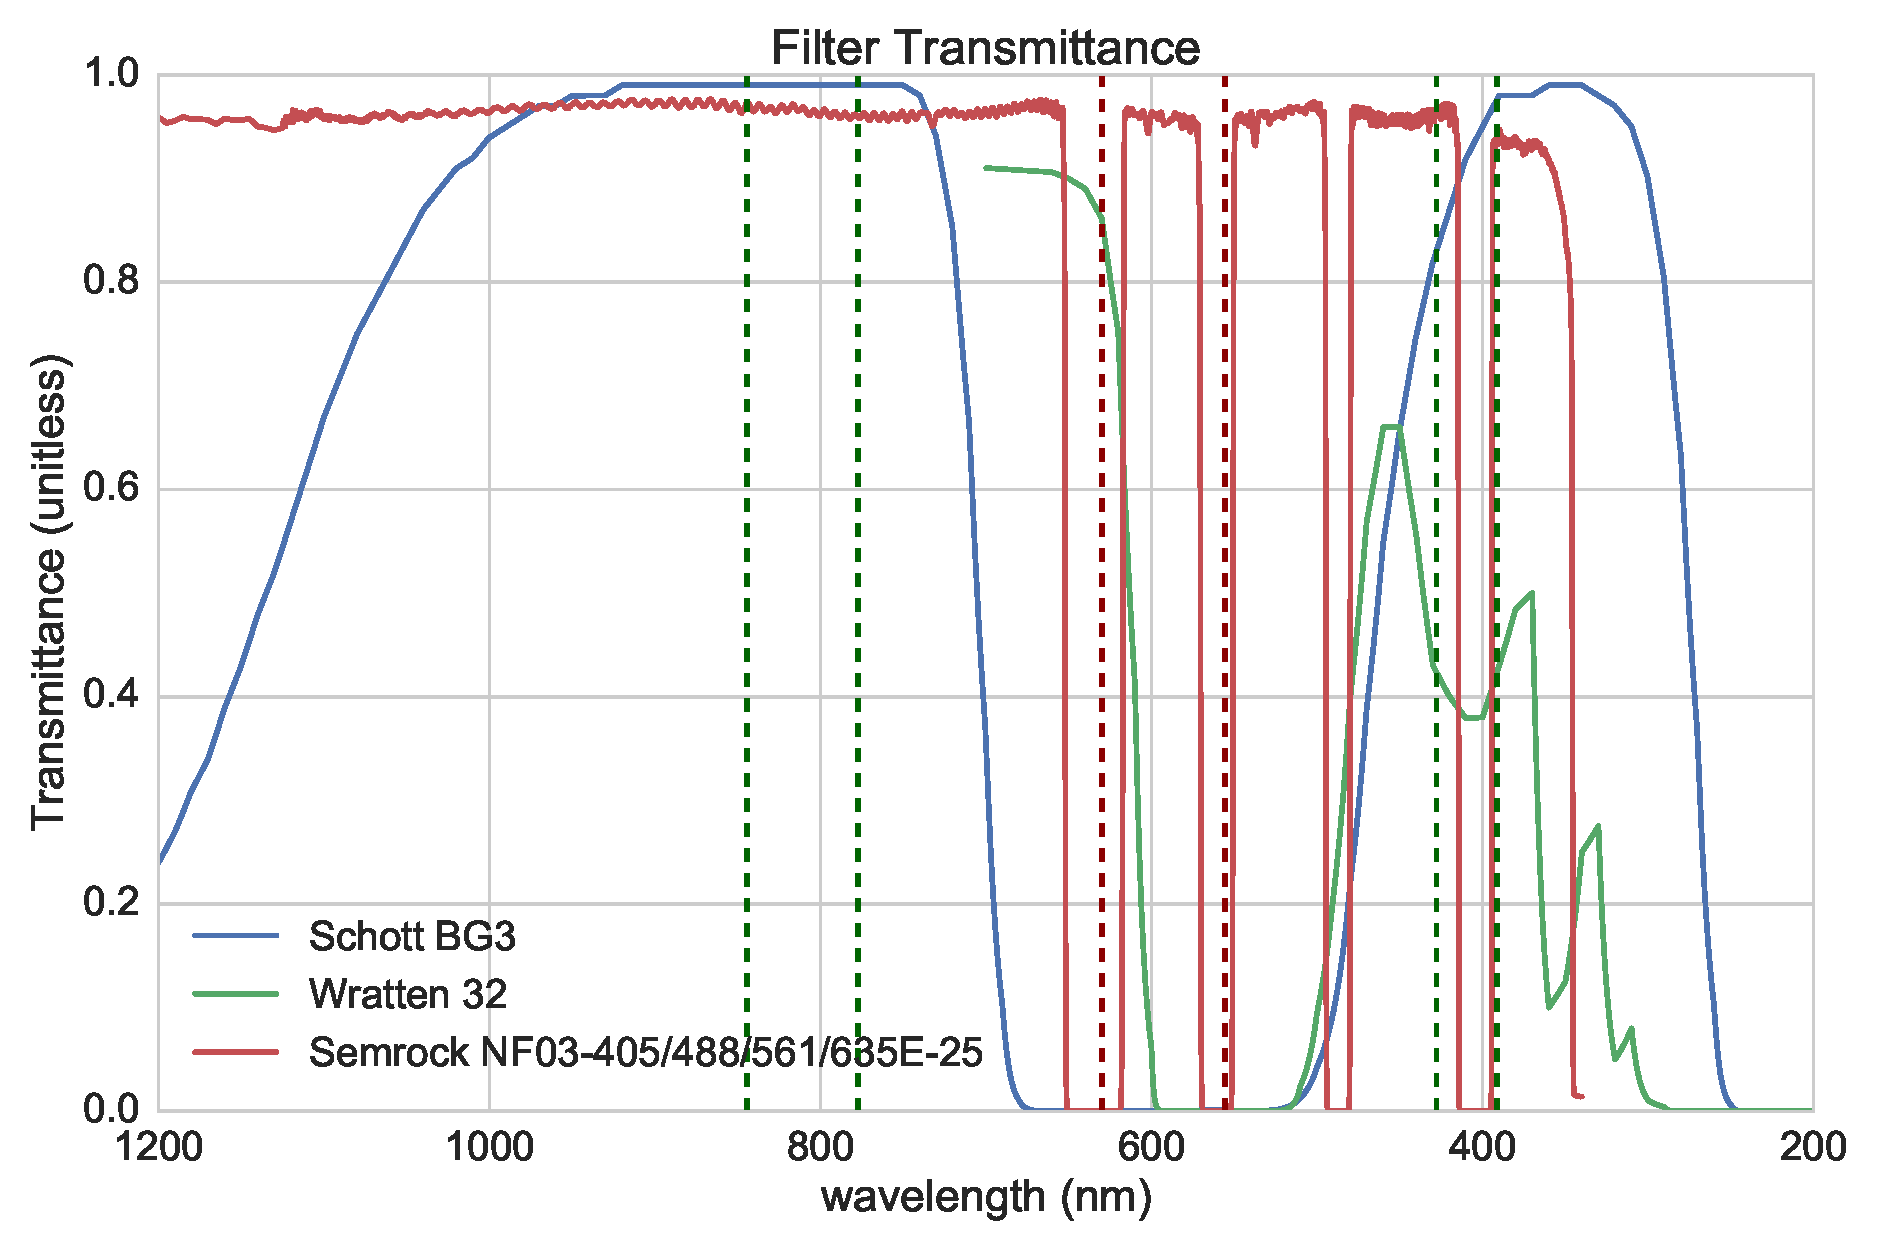
\includegraphics[width=0.9\columnwidth]{gfx/filterT}
    \caption{Comparison of bandstop filters used by other systems studying prompt auroral emissions with Schott BG3 bandstop filter used by HiST. Red markers at strong forbidden auroral emission wavelengths and green markers at strong permitted auroral emission wavelengths.}\label{fig:filters}
\end{figure}
The Wratten 32 filter \citep{wratten} has two deficiencies for fast auroral imaging: it passes the metastable oxygen emission at \unit[630]{nm} and has high attenuation of the NO emission at \unit[427.8]{nm}.
The Semrock NF03-405/488/561/635E-25 filter \citep{semrock} has similar performance \citep{jackel2014} for the auroral emissions of interest as the BG3 filters used for HiST.
HiST lenses yield a 9 degree field of view approximately centered on magnetic zenith, similar to the MOOSE instrument but HiST has significantly higher spatial resolution.
Star registration is via the astrometry.net software \citep{lang2010,hirschastro}, allowing a common local coördinate system to be created for PFISR and HiST \citep{geodata}.

The first considerations for designing a prompt auroral emissions observatory, whether based on ground, rocket or satellite include:
\begin{enumerate}
    \item Optical filtering: white light or no filtering will cover over prompt emissions with stronger, smeared forbidden emissions such as $\lambda = \unit[557.7]{nm}$, the first measured auroral emission line \citep{angstrom1869}.
    Shortpass filtering such as used in \citet{nishiyama2016} discards the medium brightness N$_2$ 1P \unit[670]{nm} and OI $\in \{777.4, 844.6\}$~nm emissions.
    Narrow-bandpass filtering discards most of the physical processes, leaving only part of the particle energy deposition picture available for estimation.
    HiST takes the bandstop filter approach, retaining most of the prompt emissions while discarding most forbidden emissions.
    \item Data inversion: remote observatories must either transmit or store data suitable for physical quantity estimation. HiST uses a unique implementation of model based iterative reconstruction (MBIR).
    MBIR reduces the dimensionality of difficult tomographic problems, thereby requiring less SNR for a given error level.
    In the medical field, MBIR is credited with reducing patient CT radiation doses by up to 98\% \citep{liu2014}.
    \item Data curation: MBIR estimation is known for being modestly time-consuming to compute.
    Currently, a single \unit[20]{ms} HiST frame takes about one minute to reconstruct a $\Phi_{top}(E,x)$ estimate \citep{hirsch2016}.
    To conserve human and computing resources, an on-site automatic data curation algorithm \citep{cviono} was developed and implemented \citep{hirsch2016bigdata}, allowing indefinite operating lifetime with yearly external USB 3.0 hard drive swap.
\end{enumerate}

Electron precipitation along $B_\parallel$ may be described by particle penetration models yielding wavelength-dependent optical intensity.
Auroral lines relevant to the filter selection of Figure~\ref{fig:filters} are listed in Table~\ref{tab:spectrum}.
\begin{table}\centering
    \caption{Selected auroral emission lines}\label{tab:spectrum}
    \begin{tabular}{rllll}
        \toprule
        $\lambda$ [nm] & family  & HiST system loss [dB] & lifetime [sec.] \\
        \midrule
        %297.2 &  [OI]31     & 13.5 & \\ % not visible due to O3 absorption (Chamberlain ch 5.1 p. 185)
        337.0 & N$_2^+$ 2P (0,0) &      &  \\
        % ~339.5 & N2+ 2P(3,6) \\
        391.4 & N$_2^+$ 1N (0,0) & 2.0  & $70 \times 10^{-9}$ \\ % high energy precip, V. Jones, 1971
        % ~394.3 & N2+ 2P(2,5) \\
        427.8 & N$_2^+$ 1N (0,1) & 1.7  & \\ % 25 R/nm
        470.9 & N$_2^+$ 1N & & \\
        486.1 & H$_\beta$ & & \\ % weak proton aurora 50-300R
        519.8, 520.0 & [NI]21 & & 1 day \\ % may be as strong as 557.7 forbidden (Chamberlain p.186)
        557.7 & [OI]32  (1s) & 28.9 & 0.74 \\ % 1190 R/nm  forbidden
        % 587.6 & He (3P-3D) & & \\ % rarely (P.E. Sandholt, Dayside and Polar Cap Aurora)
        % 589.0/589.6 & Na (2S-2P) & & \\ % occasionally (P.E. Sandholt, Dayside and Polar Cap Aurora)
        630.0 & [OI]21      & 49.7 & 107 \\  % 810R/nm forbidden
%        656.3 & H$_\alpha$ & & \\ % weak proton aurora 50-300R
        670.0 & N$_2$ 1P & &  \\ % prompt, NOT N2+
%        732.0,733.0 &    [OII] $^2$P-$^2$D & & \\ % 100eV, high altitude.  Sullivan et al
        750.0 & N$_2$ 1P & &  \\ % prompt, NOT N2+
        %761.9 &   &    & 0.9 \\ %not ground-visible: 02 absorption (Vallance Jones 1974)
        777.4 & OI   3s-3p  & 1.1 & \\  % low energy precip, quintet (chamberlain p.188) permitted
        844.6 & OI   3s-3p  & 2.3 & \\  % low energy precip, triplet permitted
        \bottomrule
    \end{tabular}
\end{table}
The temporal behavior along $B_\parallel$ help reveal the mechanism driving a particular auroral morphology.
\citet{hirsch2016} showed that using two or more tightly-synchronized high-speed cameras separated by \unit[1..10]{km} and co-aimed at magnetic zenith has high spatio-temporal resolution without the inherent ambiguities of \textit{a priori} starting altitude made necessary in single-camera studies.
Thus, DAW and inverted-V aurora for discrete arcs, even closely $B_\perp$-spaced arcs can be distinguished with HiST.

Based on rocket measurement and theory, fine spatio-temporal $B_\perp$ auroral structure comes from DAW.
HiST analysis uses a physics-based ionospheric forward model for electron precipitation in the \unit[50]{eV}..\unit[18]{keV} range with two high-speed cameras spaced \unit[3]{km} apart.
Model-based iterative reconstruction is used to estimate the differential number flux of the particles versus space and time at the top of the ionosphere.
We define the top of the ionosphere as the region below which particle acceleration is neglected and above which energy deposition is neglected.
In this manner, tightly time-synchronized camera data at \unit[30]{ms} cadence combined with ISR measurements at \unit[100]{ms} cadence yield confirming evidence for the association of DAW with strong turbulence in the lower ionosphere.

The phase 1 HiST \unit[30]{ms} observational cadence is fast enough \citep{peticolas2000,hirsch2016} to observe signatures of DAW-accelerated particle precipitating into the ionosphere.
As implied by the name, dispersive acceleration leads to higher energy particles arriving at the ionosphere first, and therefore depositing their energy in the E-region ionosphere before the lower energy particles of the same magnetospheric particle batch arrive.
The time delay between high and low energy particles is only a few hundred milliseconds \citep{dahlgren2013}, so the HiST sampling cadence gives several estimates of auroral precipitation characteristics during a dispersive impulse, sufficient to resolve key parameters of the event such as characteristic energy and beam location versus time \citep{histfeas}.


\FloatBarrier
\subsection{PFRR Digital Meridian Scanning Photometer (PDMSP)}\label{sec:pdmsp}
P-DMSP collects a six-wavelength view of intensity vs. elevation and time along the local magnetic meridian.
The meridional intensity is measured for wavelengths $\lambda \in \lbrace 427.8, 486.1, 520.0, 557.7, 630.0, 670.0 \rbrace$~nm.
The typical measurement cadence is 14 seconds, so this measurement is contextual and secondary to the primary HiST and PFISR measurements \citep{meridianreader}.
Although HiST cadence is nearly three orders of magnitude faster than P-DMSP, the spectrometer nonetheless provides temporally smeared spectral context over a wide elevation range.
A future deployment of HiST is expected to include an EMCCD-based spectrograph operating at a comparable frame rate to the full-frame HiST EMCCD imagers.